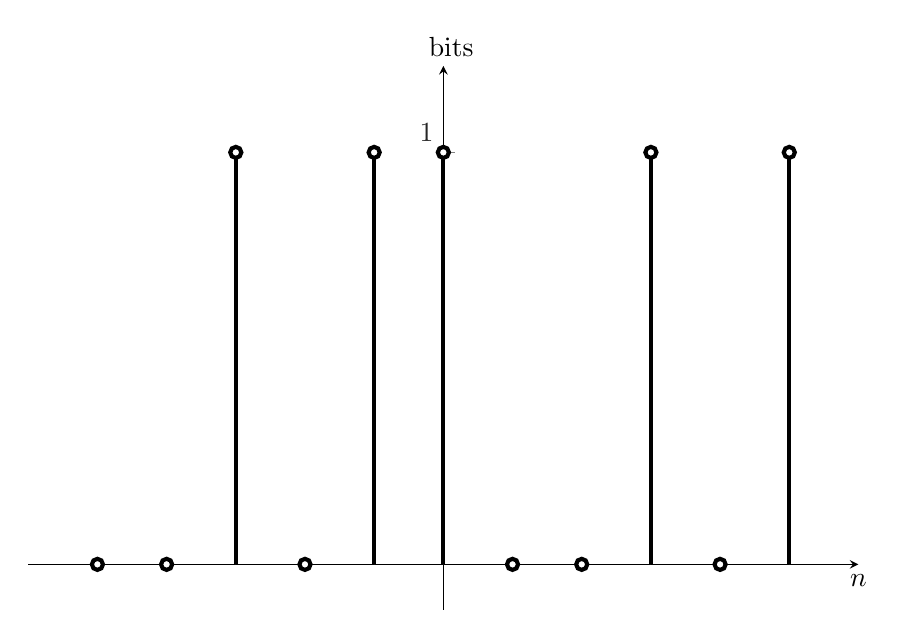
\begin{tikzpicture} 
\begin{axis}[
axis lines*=middle,
enlargelimits = true,
clip=false,
%scale only axis,
width=\textwidth,
height=0.7\textwidth,
ymin=0,
ymax=1.1,
xmin=-5,
xmax=5,
axis line style={->,>=stealth},
xlabel={$n$},
ylabel={bits},
yticklabel style = {yshift=0.25cm},
xticklabel style = {yshift=-0.1cm},
every axis x label/.style={
    at={(ticklabel* cs:1)},
    anchor=north,
},
every axis y label/.style={
    at={(ticklabel* cs:1)},
    xshift=0.1cm,
    anchor=south,
},
%xtick=\empty,
ytick={1},
xtick=\empty,
%xtick={-3.14, -1, 1, 3.14},
%xticklabels={$-\pi$, $-\omega_c$, $\omega_c$, $\pi$},
%xmajorgrids,
%ymajorgrids,
every outer y axis line/.append style={white!15!black},
every y tick label/.append style={font=\color{white!15!black}},
legend style={draw=white!15!black,fill=white,legend cell align=left}]
\pgfmathsetseed{99}
\addplot[ycomb, mark=*, fill=white, mark options={scale=1, fill=white}, line width=1.5pt, domain=-5:5, samples=11] {0.5*(sign(rand)+1)};
\end{axis}
\end{tikzpicture}
